\documentclass[fleqn,10pt,lineno]{wlpeerj}

\title{Additional details on functional boxplots \ali{a better title?}}
%  Additional details on centrality measure of epidemic functional data

\author[1]{Ali Gharouni}
\author[1,2,3]{Benjamin M. Bolker}
\affil[1]{Department of Mathematics \& Statistics, McMaster University, Hamilton, Canada}
\affil[2]{Department of Biology, McMaster University, Hamilton, Canada}
\affil[3]{Michael G. DeGroote Institute for Infectious Disease Research, McMaster University, Hamilton, Canada}
\corrauthor[1]{First Author}{agharoun@uottawa.ca \footnote{
The auther is currently at the Department of Mathematics and Statistics, University of Ottawa.}}

% \keywords{Statistical depth, Functional depth, Functional boxplot, Centroid}

\begin{abstract}
Studying the concept of \emph{central set} of an ensemble of epidemic curves -- in general functional data -- provides insights to summarize and estimate the uncertainty associated with the features of interest. These insights improve our understanding of the disease dynamics and result in reasonable forecastings. It has been argued that the classical fixed-time descriptive methods may provide unreliable estimates of centrality in functional data, specially when there exist high phase shifts among the curves. The alternative approach is to use the robust curve-based descriptive methods in which ranking process and visualizing the centrality are curvewise -- as opposed to pointwise in the fixed-time descriptive methods. We used the \emph{functional band depth} approach in our exploration of the curve-based estimation of the central set of an epidemic ensemble drawn from the output of stochastic epidemic models. We studied several \emph{statistical depths} and compared the results of the corresponding 90\% central region. We first implemented the sample-based functional band depth algorithm (FBD) with different choices of the tuning parameter $J$ to compare classical ($J=2$) with the \emph{ad hoc} ($J=50$, following \juul's 2021 approach). We then developed a multivariate generalization of ranking the curves by using Mahalanobis distance among features of interest. Further, we used the pairwise Euclidean $\ell_2$ norm to define the \emph{statistical depth}. We visually compared these methods and concluded that the classical robust FBD method (with $J=2$) and the Mahalanobis distance on features provide reasonable results \ali{thoghts?}.      
\end{abstract}

\begin{document}

\flushbottom
\maketitle
\thispagestyle{empty}

\section*{Introduction}

Summarizing features of interest and the analysis of uncertainty for ensembles of curves -- in general, functional data -- rely closely on developing robust and computationally efficient inference tools. These tools play an important role in forcasting an epidemic by summarizing different simulated temporal curves. Regardless of the generating processes of such curves, summarizing refers to computing the \emph{central set} of an ensemble. Generally speaking, there are two descriptive approaches to compute the central set; fixed-time and curve-based.

\cite{juul2021fixed} pointed out shortcomings to the standard ways that researchers draw confidence intervals for ensembles of curves, with specific examples drawn from the output of stochastic epidemic models (also, see Appendix 2 in \cite{kiss2017mathematics}'s book). In particular, they showed that fixed-time approaches (e.g., computing pointwise quantiles) can fail to capture the uncertainty in key features of an epidemic such as the timing and magnitude of epidemic peaks.  As an alternative to fixed-time approaches, the authors illustrated methods to compute the \emph{central set} of an ensemble of curves, a high-dimensional analogue of interquartile range or confidence interval. There is a large body of literature on this topic under the rubrics of \emph{functional depth} and \emph{functional boxplots} for high dimensional data \citep{fraiman2001trimmed, lopez2007depth, lopez2009concept, sun2011functional,sun2012exact}. While \juul do cite this literature \citep{sun2011functional}, exploring it in more depth led us to several useful practical and theoretical points that could be useful for researchers interested in using these approaches.

In univariate data, the central set (region) can be easily -- due to the natural ordering which allows linearly ranking the points of the dataset --represeted by the interquartile range, mean or median, and the uncertainty by confidence intervals. Classical boxplot provides a visual summary of the data with representation of centrality, uncertainty and the outlyingness. In multivariate data, computing the central set with certain uncertainty relies on the concept of \emph{statistical depth} which has several definitions \citep{mahalanobis1936generalized, tukey1975mathematics, oja1983descriptive, liu1990notion, singh1991notion, vardi2000multivariate, zuo2003projection}. This concept has been generalized to functional data, thus termed \emph{functional depth} \citep{fraiman2001trimmed}.
Roughly speaking, a statistical (functional) depth is a bounded nonnegative function which measures the average closeness of a (function) point to all other (functions) points randomly sampled, according to a distribution (for formal definitions see \citep{zuo2000general}). 
Given the concept of depth, one can order all elements of an ensemble according to decreasing depth values. This gives a ranking of the ensemble points from the \emph{center} outward. As the next canonical extention, functional boxplot was developed based on functional depth to display the data, highlight their characteristic, and reveal interesting features \citep{sun2011functional,sun2012exact}. In a recent work, \cite{wynne2021statistical} used a machine learning approache -- specifically, kernel mean embedding -- to study the functional depth.

 \cite{lopez2007depth} developed functional band depth (FBD) which is a sample-based method for determining a curve's centrality (and hence whether it should be included in a central set of curves for display). It measures the fraction of times that a given curve is completely included within the envelope of a set of other curves randomly sampled from the ensemble. The sample size is determined by a \emph{tuning parameter} denoted by $J$, and the number of samples is determined by all possible combinations. In a comparable approach to FBD algorithm, \juul primarily studied the curve centrality on an epidemic ensemble. They chose the \emph{tuning parameter} as $J=50$ (they use the notation \ncurve), and chose $\nsample=100$ such samples to compute the fraction (\emph{band depth}) for each curve. They provided open-source Python code that implements this method, as well as some of the weighted variants they discuss. For the simple (unweighted) case, however, there are already mature open source implementations available in R \citep{fda_pkg,roahd}, Matlab (\url{https://www.psych.mcgill.ca/misc/fda/downloads/FDAfuns/}), and Python \citep{seabold2010statsmodels}. In general these packages use the same functional band depth measure as \juul, but substituting $J=2$, which is robust \citep{lopez2009concept} and allows the use of a computationally efficient algorithm for large data sets \citep{sun2012exact}. It is unclear why \juul chose larger values of $J$ (10 and 50), although the dimensions of their examples are small enough that the computational burden is not important.

\juul also suggest ranking according to a single, one-dimensional feature of interest such as the maximum values of newly hospitalized cases in a single day (their Fig.~2e). We suggest that this approach could be extended to incorporate multiple features of interest. Functional band depth could again be used on this reduced set of features; here we use the \emph{Mahalanobis distance} \citep{mahalanobis1936generalized}, which measures distance from a centroid accounting both for variation in the scales or typical magnitudes of different features and for correlation among features. Our example uses a feature set including the peak value of incidence (new infections), the time at which the peak occurs, and the initial growth rate, duration, and final size of the epidemic. While these are typical epidemiological features of interest, researchers can and should choose the features that are most closely connected to their particular research questions \citep{probert2016decision}.

In this work, we explore \juul's curve-based statistical approach in more depth which led us to several useful practical and theoretical points that could be useful for researchers interested in using these approaches. In particular, we compare the central set of the epidemic ensemble (provided in \juul's work) by defining various statistical depths and ranking the curves following (i) functional band depth algorithm (FBD) with different choices of the tuning parameter $J$ to compare classical ($J=2$) with \juul's 2021 approach ($J=50$), (ii) Mahalanobis distance among features of interest, and (iii) pairwise Euclidean $\ell_2$ norm. Although we used an epidemic ensemble, but our method can be used in general setting.

\section*{Methods}

In this work, we present the comparison of 90\% central regions computed with different functional band depth methods. We apply our methods on \juul dataset (\url{https://github.com/jonassjuul/curvestat/tree/master/curvestat/tests/test_data}) and compare our results with theirs.

First, we implemented \juul's primary sampling-based method in R \citep{R} for determining a curve's centrality which in nature is similar to FBD with differences in sampling size and number of samples. In particular, the implemented algorithm involves the following steps: (i) a subset of curves was randomly sample from the ensemble (FBD: J=2, \juul : J=50), (ii) compute the sample-specific min-max envelopes, (iii) score individual curves based on whether they lie entirely within the envelope (thus, score=1) or not (thus, score=0), and (vi) repeat to derive a centrality scoring or ``rank'' on [0,1] for each curve based on the proportion. In particular, the curve-specific ``rank'' is estimated by the `median-like' criterion (sumation of scores). The ``central region'', specifically 90\% central region, is characterized as the region containing the most central curves with their ranks $> 0.1$ quantile.

Secondly, we used the function fda() in R \citep{R} package \pkg{roahd} \citep{roahd}, with the choice of modified band depth (MBD) to break ties which is based on the fast algorithm proposed by \cite{sun2012exact}. Likewise the implemented method in previous step, the curve-specific ranks are sorted and the ``central'' region was ploted. 

Thirdly, for an individual curve in the ensemble, a feature vector was assigned. The curves are ranked according to thier feature vector. Specifically, we used function mahalanobis() in R \citep{R} to compute the pairwise Mahalanobis distance between the features of two curves with the covariance matrix from the entire data set as the scaling factor. This is because we can't compute the covariance matrix for only two samples. In this case, the rank of each curve is the average distance to the rest of the set. The 90\% central region is considered as curves with ranks $< 0.9$ quantile. Note that, the following features of interest were chosen for each curve in the ensemble; (i) the peak value of incidence (specifically, new infections), (ii) the time at which the peak occurs, (iii) the initial growth rate, (iv) epidemic duration, and (v) final size of the epidemic. Specifically, the peak was determined by the global maximum of a curve on its domain. The initial growth rate was estimated by fitting an exponential function to the section of the curve starting from the first day of nonzero prevalence to the day when the prevalence is 10\%. The epidemic duration was determinded by the time between 10\% and 90\% prevalence cumulative cases. The final size was given by the integration of the curve over time.


\section*{Results}

The 90\% central regions computed with both pairwise Mahalanobis distance approach and FBD with $J=2$ are comparable with \juul's result, i.e., FBD with $J=50$. It appears that both pairwise Mahalanobis distance approach and FBD with $J=2$ identify an earlier peak as being part of the central set while in general \juul's result may be shifted by 1 index point relative to other two.

\begin{figure}[ht]\centering
  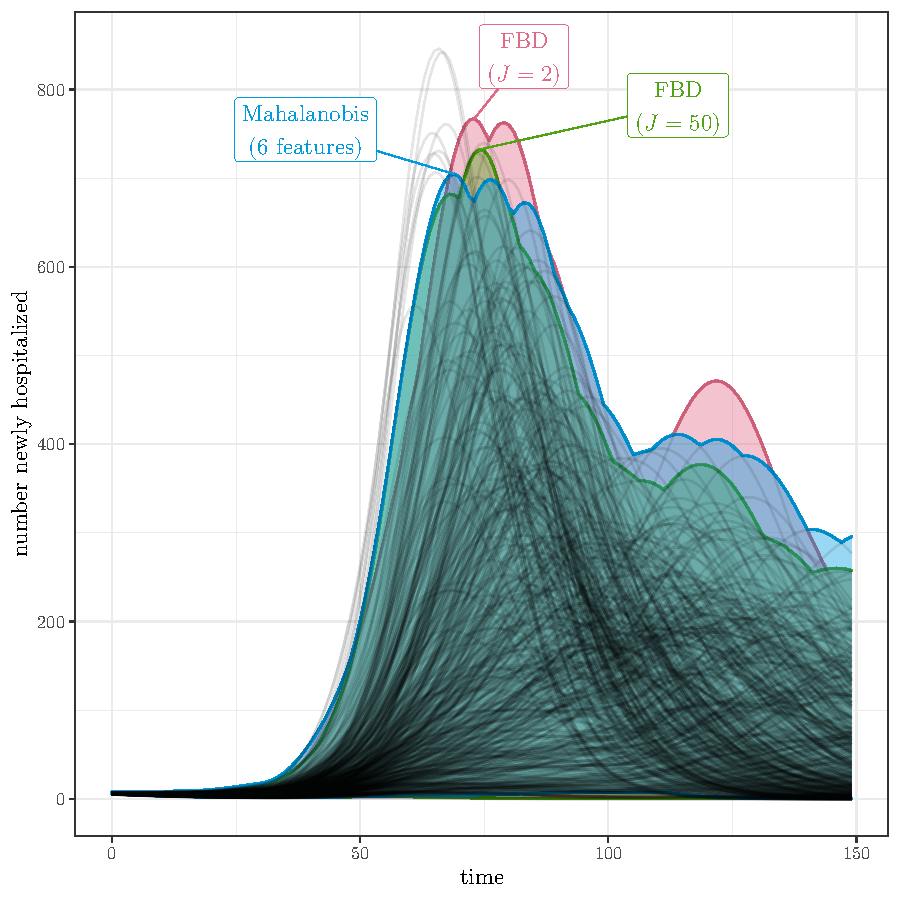
\includegraphics[width=\linewidth]{scripts/cent_plot.pdf}
  \caption{Comparison of 90\% central regions computed with
    different functional boxplot methods, using epidemic curve ensembles from \juul. FBD = functional band distance; $J$ = number of curves used for centrality calculation. Curve with $J=2$ computed via the \texttt{roahd} package \citep{roahd}: curve with $J=50$ used our own implementation of the functional band distance algorithm described by \juul, curve with Mahalanobis (5 features) used Mahalanobis distance on features of interest including the peak value of incidence, the time at which the peak occurs, the initial growth rate, epidemic duration, and final size of the epidemic.
  }
  \label{p.a}
\end{figure}
 
\section*{Discussion}

In our exploration of estimating the \emph{central set} -- also refer to as ``centroid'' -- out of an ensemble of curves, we compared applying measures of centrality directly to the curves versus to features derived from the curves. In this work, we are computing the ``most central'' point in the set which we characterize as the point with minimum distance to all other points. The ``most central'' point is different from the concept of ``centroid''. In particular, in a space for a rank $r$, the (1) set of $r$ closest points to the centroid is can be estimated (2) the set of $r$ points with the minimum average distance to all of the other points. We note that these two concepts can be different with respect to the choice of the norm, e.g., log Euclidean norm.

In our multivariate generalization of ranking the curves based on features derived from the curves, we used Mahalanobis distance on feature vectors. We note that one potential problem with Mahalanobis distances is if (for example) the feature distribution is strongly bimodal, then scaling factors/correlations derived from the overall data set may not be appropriate for scaling the components of distance between two trajectories whose features put them in the same mode/component of the distribution.

We also implemented a pairwise-distance approach, i.e., pairwise distances between the curves and quantiles of centrality, as an alternative method to a sampling-based functional boxplot. In particular, we compute all pairwise distances -- here we used $\ell_2$ norm which gives the area between the two curves -- between the curves, determine the median-like distance of a curve to all others as the minimum of sum of distances, and estimate the distribution of distances. We compared the 90\% most central region using the $\ell_2$ norm with the results from sampling-based method FBD and our proposed ranking method using Mahalanobis distance among features of interest (see appendix). We concluded that pairwise-distance approach using $\ell_2$ norm underestimated the key features of epidemic ensemble such as the magnitude of epidemic peaks. Further, and alongside testing the Euclidean $\ell_2$ norm, on the pairwise curves, we considered other classic curve distances like Fréchet and dynamic time warping (DTW). It is notable that these norms ignore phase differences and sound inappropriate for the purpose of centrality measure in this dataset.

\section*{Conclusions}

\section*{Acknowledgments}

\bibliography{./curveBP}

\section*{Appendix}

% FIXME: change L_2 to \ell_2
\begin{figure}[ht]\centering
  \includegraphics[width=\linewidth]{scripts/cent_plot2.pdf}
  \caption{Comparison of 90\% central regions computed with
    different functional boxplot and pairwise-distance methods, using epidemic curve ensembles from \juul. FBD = functional band distance; $J$ = number of curves used for centrality calculation. Curve with $J=2$ computed via the \texttt{roahd} package \citep{roahd}, curve with $J=50$ used our own implementation of the functional band distance algorithm described by \juul, curve with Mahalanobis (5 features) used Mahalanobis distance on features of interest including the peak value of incidence, the time at which the peak occurs, the initial growth rate, epidemic duration, and final size of the epidemic. Curve with $\ell_2$ used  pairwise $\ell_2$ distances between the curves and determinded quantiles of centrality.
  }
  \label{p.b}
\end{figure}
\end{document}